\documentclass[11pt,tikz]{standalone}

\begin{document}

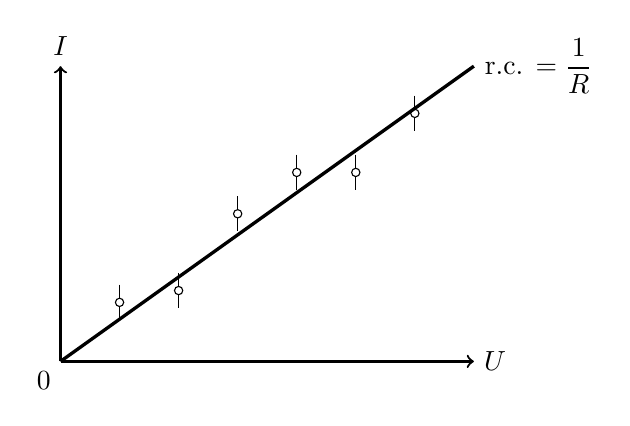
\begin{tikzpicture}[scale=.75]
  % \clip (-1em, -1.2em) rectangle (8, 5.5);
  \foreach \pos in {(1, 1), (2, 1.2), (3, 2.5), (4, 3.2), (5, 3.2), (6, 4.2)} {
      \draw \pos +(0, .3) -- +(0, -.3);
      \draw[fill=white] \pos circle (2pt);
    }
  \draw[very thick, domain=0:7] plot (\x, 5 / 7 * \x) node[right] {r.c. $\displaystyle = \frac{1}{R}$};
  \draw[->, thick] (0, 0) -- (7, 0) node[right] {$U$};
  \draw[->, thick] (0, 0) -- (0, 5) node[above] {$I$};
  \node[below left] at (0, 0) {0};
\end{tikzpicture}

\end{document}